% Options for packages loaded elsewhere
\PassOptionsToPackage{unicode}{hyperref}
\PassOptionsToPackage{hyphens}{url}
%
\documentclass[
]{article}
\title{Oxford : Smooth fit to log-odds ratios}
\author{Vincent Guitteny, Freddie Joly, Tom Léchappé et Elyes Zribi}
\date{06 avril 2022}

\usepackage{amsmath,amssymb}
\usepackage{lmodern}
\usepackage{iftex}
\ifPDFTeX
  \usepackage[T1]{fontenc}
  \usepackage[utf8]{inputenc}
  \usepackage{textcomp} % provide euro and other symbols
\else % if luatex or xetex
  \usepackage{unicode-math}
  \defaultfontfeatures{Scale=MatchLowercase}
  \defaultfontfeatures[\rmfamily]{Ligatures=TeX,Scale=1}
\fi
% Use upquote if available, for straight quotes in verbatim environments
\IfFileExists{upquote.sty}{\usepackage{upquote}}{}
\IfFileExists{microtype.sty}{% use microtype if available
  \usepackage[]{microtype}
  \UseMicrotypeSet[protrusion]{basicmath} % disable protrusion for tt fonts
}{}
\makeatletter
\@ifundefined{KOMAClassName}{% if non-KOMA class
  \IfFileExists{parskip.sty}{%
    \usepackage{parskip}
  }{% else
    \setlength{\parindent}{0pt}
    \setlength{\parskip}{6pt plus 2pt minus 1pt}}
}{% if KOMA class
  \KOMAoptions{parskip=half}}
\makeatother
\usepackage{xcolor}
\IfFileExists{xurl.sty}{\usepackage{xurl}}{} % add URL line breaks if available
\IfFileExists{bookmark.sty}{\usepackage{bookmark}}{\usepackage{hyperref}}
\hypersetup{
  pdftitle={Oxford : Smooth fit to log-odds ratios},
  pdfauthor={Vincent Guitteny, Freddie Joly, Tom Léchappé et Elyes Zribi},
  hidelinks,
  pdfcreator={LaTeX via pandoc}}
\urlstyle{same} % disable monospaced font for URLs
\usepackage[margin=1in]{geometry}
\usepackage{graphicx}
\makeatletter
\def\maxwidth{\ifdim\Gin@nat@width>\linewidth\linewidth\else\Gin@nat@width\fi}
\def\maxheight{\ifdim\Gin@nat@height>\textheight\textheight\else\Gin@nat@height\fi}
\makeatother
% Scale images if necessary, so that they will not overflow the page
% margins by default, and it is still possible to overwrite the defaults
% using explicit options in \includegraphics[width, height, ...]{}
\setkeys{Gin}{width=\maxwidth,height=\maxheight,keepaspectratio}
% Set default figure placement to htbp
\makeatletter
\def\fps@figure{htbp}
\makeatother
\setlength{\emergencystretch}{3em} % prevent overfull lines
\providecommand{\tightlist}{%
  \setlength{\itemsep}{0pt}\setlength{\parskip}{0pt}}
\setcounter{secnumdepth}{5}
\usepackage{stmaryrd} \usepackage{float} \floatplacement{figure}{H}
\ifLuaTeX
  \usepackage{selnolig}  % disable illegal ligatures
\fi

\begin{document}
\maketitle

\newenvironment{cols}[1][]{}{}
\newenvironment{col}[1]{\begin{minipage}{#1}\ignorespaces}{%
\end{minipage}
\ifhmode\unskip\fi
\aftergroup\useignorespacesandallpars}
\def\useignorespacesandallpars#1\ignorespaces\fi{%
#1\fi\ignorespacesandallpars}
\makeatletter
\def\ignorespacesandallpars{%
  \@ifnextchar\par
    {\expandafter\ignorespacesandallpars\@gobble}%
    {}%
}
\makeatother

\renewcommand\contentsname{Table des matières}
\newpage
\tableofcontents
\newpage

\hypertarget{pruxe9sentation-du-jeu-de-donnuxe9es}{%
\section{Présentation du jeu de
données}\label{pruxe9sentation-du-jeu-de-donnuxe9es}}

L'objectif de cette étude est d'observer l'influence que peut avoir
l'exposition d'une mère aux rayons X pendant sa grossesse sur les décés
des enfants par un cancer (de 0 à 9 ans). Les données sont séparées en
120 jeux de données en fonction de l'âge de l'enfant de son année de
naissance (1944-1964). Dans notre cas, seule l'influence de l'année de
naissance est retenue. Ces valeurs varient de \(-10\) à \(10\) en
prenant en compte que \(0\) correspond à l'année 1954. Pour chacune des
120 partitions, on dispose du nombre de décés \(r\) parmi une population
de \(n\) enfants pour deux groupes :

\begin{itemize}
\tightlist
\item
  un groupe d'enfants dont les mères ont été exposées à des rayons X au
  cours de leur grossesse
\item
  un groupe ``témoin'' dont les mères n'ont pas été exposées.
\end{itemize}

\hypertarget{pruxe9sentation-du-moduxe8le}{%
\section{Présentation du modèle}\label{pruxe9sentation-du-moduxe8le}}

Regardons maintenant le modèle proposé par les auteurs. Pour chaque
strate \(i\) et pour les deux groupes de population, le nombre de décés
est donné par une loi binomiale :

\begin{itemize}
\tightlist
\item
  \(r_i^0 \sim Bin(n_i^0,p_i^0)\)
\item
  \(r_i^1 \sim Bin(n_i^1,p_i^1)\).
\end{itemize}

Ainsi les paramètres \(p_i^0\) et \(p_i^1\) sont donnés par les deux
formules suivantes :

\begin{itemize}
\tightlist
\item
  \(p_i^0 = sigmoid(\mu_i)\)
\item
  \(p_i^1 = sigmoid(\mu_i+\alpha+\beta_1 year_i+\beta_2(year_i^2-22)+b_i)\)
  ou bien \(p_i^1 = sigmoid(\mu_i+log\psi_i)\) où
  \(log\psi_i = \alpha+\beta_1 year_i+\beta_2(year_i^2-22)+b_i\).
\end{itemize}

Le paramètre \(b_i\) suit une loi normale \(\mathcal N(0,\sigma^2)\).

Il reste donc les lois ``non informatives'' des paramètres suivants :

\begin{itemize}
\tightlist
\item
  \(\alpha \sim\mathcal N(0,\sigma_{\alpha}^2)\)
\item
  \(\beta_1 \sim\mathcal N(0,\sigma_{\beta_1}^2)\)
\item
  \(\beta_2 \sim\mathcal N(0,\sigma_{\beta_2}^2)\)
\item
  \(\sigma^2 \sim InvGamma(a_{\sigma},b_{\sigma})\)
\item
  \(\mu_i \sim\mathcal N(0,\sigma_{\mu}^2)\).
\end{itemize}

On représente le modèle hiérarchique sous la forme d'un graphe
ci-dessous.

\begin{figure}
\centering
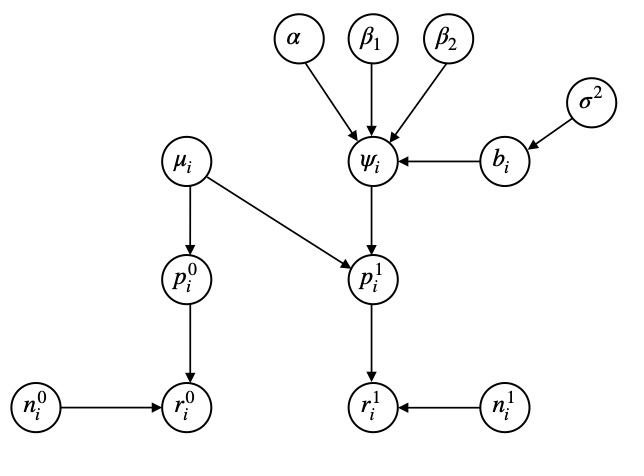
\includegraphics[width=0.5\textwidth,height=\textheight]{Model.jpg}
\caption{Modèle hierarchique}
\end{figure}

\hypertarget{calculs-des-lois-conditionnelles-pleines}{%
\section{Calculs des lois conditionnelles
pleines}\label{calculs-des-lois-conditionnelles-pleines}}

On veut maintenant calculer les lois conditionnelles pleines de nos
paramètres afin de mettre en oeuvre un échantilloneur de Gibbs sur ce
modèle. Bien que la loi conditionnelle pleine de \(\sigma^2\) soit
identifiable, celles des autres paramètres ne sont pas identifiables. On
donne ici un exemple de calcul pour le paramètre \(\alpha\), les autres
calcul sont donnés en annexe. Les noeuds de notre modèle représentés par
\(log(\psi_i)\), \(p_i^0\) et \(p_i^1\) étant non stochastiques dans
notre modèle, on peut les ignorer lors du calcul des lois
conditionnelles pleines.

\hypertarget{calcul-pour-sigma2}{%
\subsection{\texorpdfstring{Calcul pour
\(\sigma^2\)}{Calcul pour \textbackslash sigma\^{}2}}\label{calcul-pour-sigma2}}

On calcule la loi conditionnelle pleine du paramètre \(\sigma^2\).

\begin{align*}
\Pi(\sigma^2|...) &\propto \Pi(\sigma^2) \prod_{i=1}^n\Pi(b_i|\sigma^2) \\
&\propto \exp\left({\frac{-b_{\sigma}}{\sigma^2}}\right)(\sigma^2)^{-a_{\sigma}-1}\prod_{i=1}^{n} \exp\left(\frac{-b_i^2}{2\sigma^2}\right)(\sigma^2)^{-\frac{1}{2}} \\
&\propto (\sigma^2)^{-a_{\sigma}-1-\frac{n}{2}} \exp\left(\frac{-2b_{\sigma}-\sum\limits_{i=1}^n b_i^2}{2\sigma^2}\right)
\end{align*}

Ainsi, on identifie une loi inverse gamma :

\begin{align*}
\Pi(\sigma^2|...) &\sim InvGamma(\frac{n}{2}+a_{\sigma},\frac{2b_{\sigma}+\sum\limits_{i=1}^n b_i^2}{2})
\end{align*}

\hypertarget{exemple-de-calcul-pour-une-loi-non-identifiable}{%
\subsection{Exemple de calcul pour une loi non
identifiable}\label{exemple-de-calcul-pour-une-loi-non-identifiable}}

On calcule la loi conditionnelle pleine du paramètre \(\alpha\).

\begin{align*}
\Pi(\alpha|...) &\propto \Pi(\alpha) \prod_{i=1}^n\Pi(r_i^1|...) \\
&\propto \exp\left({\frac{-\alpha^2}{2\sigma_{\alpha}^2}}\right)\prod_{i=1}^n \left((p_i^1)^{r_i^1}(1-p_i^1)^{n_i^1-r_i^1}\right)
\end{align*}

où \(p_i^0=sigmoid(\mu_i)\) et
\(p_i^1=sigmoid(\mu_i+\alpha+\beta_1 year_i+\beta_2(year_i^2-22)+b_i)\).

\hypertarget{impluxe9mentation-et-ruxe9sultats}{%
\section{Implémentation et
résultats}\label{impluxe9mentation-et-ruxe9sultats}}

\hypertarget{annexe}{%
\section{Annexe}\label{annexe}}

\hypertarget{loi-conditionnelle-pleine-du-paramuxe8tre-beta_1}{%
\subsection{\texorpdfstring{Loi conditionnelle pleine du paramètre
\(\beta_1\)}{Loi conditionnelle pleine du paramètre \textbackslash beta\_1}}\label{loi-conditionnelle-pleine-du-paramuxe8tre-beta_1}}

\begin{align*}
\Pi(\beta_1|...) &\propto \Pi(\beta_1) \prod_{i=1}^n\Pi(r_i^1|...) \\
&\propto \exp\left({\frac{-\beta_1^2}{2\sigma_{\beta_1}^2}}\right)\prod_{i=1}^n \left((p_i^1)^{r_i^1}(1-p_i^1)^{n_i^1-r_i^1}\right)
\end{align*}

\hypertarget{loi-conditionnelle-pleine-du-paramuxe8tre-beta_2}{%
\subsection{\texorpdfstring{Loi conditionnelle pleine du paramètre
\(\beta_2\)}{Loi conditionnelle pleine du paramètre \textbackslash beta\_2}}\label{loi-conditionnelle-pleine-du-paramuxe8tre-beta_2}}

\begin{align*}
\Pi(\beta_2|...) &\propto \Pi(\beta_2) \prod_{i=1}^n\Pi(r_i^1|...) \\
&\propto \exp\left({\frac{-\beta_2^2}{2\sigma_{\beta_2}^2}}\right)\prod_{i=1}^n \left((p_i^1)^{r_i^1}(1-p_i^1)^{n_i^1-r_i^1}\right)
\end{align*}

\hypertarget{loi-conditionnelle-pleine-du-paramuxe8tre-b_i}{%
\subsection{\texorpdfstring{Loi conditionnelle pleine du paramètre
\(b_i\)}{Loi conditionnelle pleine du paramètre b\_i}}\label{loi-conditionnelle-pleine-du-paramuxe8tre-b_i}}

\begin{align*}
\Pi(b_i|...) &\propto \Pi(b_i|\sigma^2) \Pi(r_i^1|...) \\
&\propto \exp\left({\frac{-b_i^2}{2\sigma^2}}\right) \left((p_i^1)^{r_i^1}(1-p_i^1)^{n_i^1-r_i^1}\right)
\end{align*}

\hypertarget{loi-conditionnelle-pleine-du-paramuxe8tre-mu_i}{%
\subsection{\texorpdfstring{Loi conditionnelle pleine du paramètre
\(\mu_i\)}{Loi conditionnelle pleine du paramètre \textbackslash mu\_i}}\label{loi-conditionnelle-pleine-du-paramuxe8tre-mu_i}}

\begin{align*}
\Pi(\mu_i|...) &\propto \Pi(\mu_i)\Pi(r_i^0|\mu_i)\Pi(r_i^1|...) \\
&\propto \exp\left({\frac{-\mu_i^2}{2\sigma_{\mu}^2}}\right)\left((p_i^0)^{r_i^0}(1-p_i^0)^{n_i^0-r_i^0}\right)\left((p_i^1)^{r_i^1}(1-p_i^1)^{n_i^1-r_i^1}\right)
\end{align*}

\end{document}
